\part{Transformations}
\frame{\partpage}

\begin{frame}{Right hand rule}
	\pause OpenGL uses a \textbf{right-handed coordinate system}
	\pause \begin{center}
		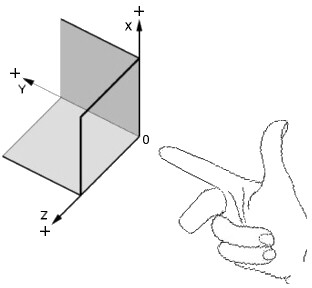
\includegraphics[width=0.3\textwidth]{RightHandRule}
	\end{center}
	\begin{itemize}
		\pause\item The \textbf{$x$-axis} points towards the \textbf{right-hand side} of the screen
		\pause\item The \textbf{$y$-axis} points towards the \textbf{top} of the screen
		\pause\item The \textbf{$z$-axis} points \textbf{out} of the screen
	\end{itemize}
\end{frame}

\begin{frame}{Transformations and matrices}
	\begin{itemize}
		\pause\item A \textbf{transformation} is a \textbf{mathematical function} that \textbf{changes points in space}
		\pause\item E.g.\ shifts them, rotates them, scales them, ...
		\pause\item Many useful transformations can be \textbf{represented} by matrices
		\pause\item Multiplying these matrices together \textbf{combines} the transformations
		\pause\item Multiplying a vector by the matrix \textbf{applies} the transformation
	\end{itemize}
\end{frame}

\begin{frame}[fragile]{GLM}
	\begin{itemize}
		\pause\item We will use the \textbf{GLM} library to do matrix calculations for us
		\pause\item \url{http://glm.g-truc.net/}
		\pause\item GLM aims to mirror GLSL data types (\lstinline{vec4}, \lstinline{mat4} etc) in C++
		\pause\item Lets us perform calculations with vectors and matrices in C++
		\pause\item GLM types can be passed into shaders as uniforms, e.g.
			\begin{lstlisting}
// transformLocation points to a uniform of type mat4
glm::mat4 transform = ...;
glUniformMatrix4fv(transformLocation, 1, GL_FALSE, glm::value_ptr(transform));
			\end{lstlisting}
	\end{itemize}
\end{frame}

\begin{frame}[fragile]{Identity}
	\pause The identity transformation does not change anything
	\pause \begin{lstlisting}
// Default constructor for glm::mat4 creates an identity matrix
glm::mat4 transform;
	\end{lstlisting}
\end{frame}

\begin{frame}[fragile]{Translation}
	\pause Translation shifts all points by the same vector offset
	\pause \begin{lstlisting}
transform = glm::translate(transform, glm::vec3(0.3f, 0.5f, 0.0f));
	\end{lstlisting}
\end{frame}

\begin{frame}[fragile]{Scaling}
	\pause Scaling moves all points closer or further from the origin by the same factor
	\pause \begin{lstlisting}
transform = glm::scale(transform, glm::vec3(1.2f, 0.5f, 1.0f));
	\end{lstlisting}
\end{frame}

\begin{frame}[fragile]{Rotation}
	\begin{itemize}
		\pause\item How do we represent a rotation in 3 dimensions?
		\pause\item One way is by specifying the \textbf{axis} (as a vector) and the \textbf{angle} (in radians)
		\pause\item Axis always runs through the origin
	\end{itemize}
	\pause \begin{lstlisting}
float angle = glm::pi<float>() * 0.5f;
glm::vec3 axis(0, 0, 1);
transform = glm::rotate(transform, angle, axis);
	\end{lstlisting}
\end{frame}

\begin{frame}[fragile]{Combining transformations}
	\pause \begin{lstlisting}
transform = glm::translate(transform, glm::vec3(0.5f, 0.5f, 0.0f));
transform = glm::rotate(transform, angle, axis);
	\end{lstlisting}
	\begin{itemize}
		\pause\item Transformations \textbf{do not commute} in general ---
			changing the order will change the result
		\pause\item The order they are applied is the \textbf{reverse} of what you might think ---
			i.e.\ the above rotates \textbf{then} translates
	\end{itemize}
\end{frame}

\begin{frame}{The model matrix}
	\pause Exactly what we've been doing so far today...
\end{frame}

\begin{frame}[fragile]{The view matrix}
	\pause Need to translate and rotate the scene so that the ``camera'' is at $(0,0,0)$ and looking in the negative $z$ direction
	\pause\begin{lstlisting}
glm::mat4 view = glm::lookAt(
  glm::vec3(2, 0, 2),    // eye
  glm::vec3(0, 0, 0),    // centre
  glm::vec3 up(0, 1, 0)  // up
);
	\end{lstlisting}
	\begin{itemize}
		\pause\item \lstinline{eye} is the position of the camera
		\pause\item \lstinline{centre} is a point for the camera to look at
		\pause\item \lstinline{up} is which direction is ``up'' for the camera (usually the positive $y$-axis)
	\end{itemize}
\end{frame}

\begin{frame}[fragile]{The projection matrix}
	\pause\begin{lstlisting}
glm::mat4 projection = glm::perspective(
	glm::radians(45.0f), // field of view
	4.0f / 3.0f,         // aspect ratio
	0.1f,                // near clip plane
	100.0f               // far clip plane
);
	\end{lstlisting}
	\begin{itemize}
		\pause\item \textbf{Field of view (FOV)}: how ``wide'' or ``narrow'' the view is
		\pause\item \textbf{Aspect ratio}: should be \lstinline{screenWidth / screenHeight}
		\pause\item \textbf{Near and far clip planes}: fragments that fall outside this range of distances from the camera are not drawn
	\end{itemize}
	\pause Also available: \lstinline{glm::ortho} for orthographic projection
\end{frame}